
%(BEGIN_QUESTION)
% Copyright 2015, Tony R. Kuphaldt, released under the Creative Commons Attribution License (v 1.0)
% This means you may do almost anything with this work of mine, so long as you give me proper credit

En sikkerhetsinnretning som ofte monteres på prosessbeholdere med trykksatt gass er en {\it Pressure Safety Valve}, eller PSV. I dette eksemplet beskytter en PSV en reaktorbeholder mot brudd på grunn av for høyt internt gasstrykk. PSV-en er satt til å åpne (``lift'') og avlaste tanken dersom det interne trykket overstiger 77 PSI:

$$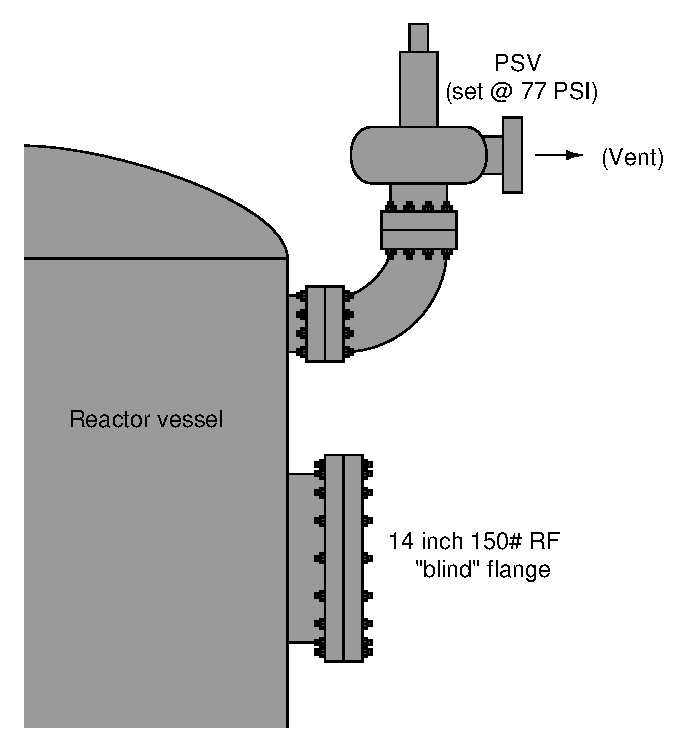
\includegraphics[width=15.5cm]{i00502x01.eps}$$

Beregn den totale kraften som virker på en 14 tommers blindflens på siden av reaktoren ved PSV-ens åpningstrykk, både i pund og i tonn. Bruk 13$1 \over 4$ tommer som effektiv diameter for blindflensen.

\vskip 10pt

$F_{total}$ = \underbar{\hskip 50pt} lb

\vskip 10pt

$F_{total}$ = \underbar{\hskip 50pt} tons

\vskip 20pt \vbox{\hrule \hbox{\strut \vrule{} {\bf Forslag til sokratisk diskusjon} \vrule} \hrule}

\begin{itemize}
\item{} Dersom reaktorbeholderen inneholdt væske i stedet for gass, ville det påvirket kraftberegningen på flensen? Hvorfor eller hvorfor ikke?
\item{} Dersom reaktorbeholderen inneholdt væske i stedet for gass, ville det påvirket riktig valg av overtrykksventil? Hvorfor eller hvorfor ikke?
\item{} Dersom temperaturen i reaktorbeholderen økte betydelig, ville det påvirket riktig innstilling av overtrykksventilen? Hvorfor eller hvorfor ikke?
\item{} Dersom fluidet i reaktoren var svært brannfarlig og/eller giftig, hva ville vært den sikreste måten å rørføre en overtrykksventil på, siden direkte utslipp til atmosfæren i seg selv ville vært utrygt?
\item{} En farlig praksis som dessverre finnes i enkelte industrier kalles {\it hot-bolting} av flenser, der bare halvparten av flensboltene (altså annenhver bolt) strammes for å holde flensen på plass under oppstart. Forklar hvorfor denne praksisen er uforsvarlig, og forklar også hvilke forhold som kan friste driftsoperatører til å gjøre dette.
\end{itemize}

\underbar{file i00502}
%(END_QUESTION)





%(BEGIN_ANSWER)


%(END_ANSWER)





%(BEGIN_NOTES)

$$F = PA$$

$$F = P \pi r^2$$

$$F_{total} = (77 \hbox{ PSI}) \pi (13.25 \hbox{ in} / 2)^2$$

$$F_{total} = (77 \hbox{ PSI}) \pi (6.625 \hbox{ in})^2$$

$$F_{total} = (77 \hbox{ PSI}) (137.89 \hbox{ in}^2)$$

$$F_{total} = 10,617 \hbox{ lb} = 5.309 \hbox{ tons}$$

%INDEX% Physics, fluids: pressure, force, and area
%INDEX% Physics, units and conversions: pressure
%INDEX% Safety, pressure protection: safety valve

%(END_NOTES)

